\documentclass[./main.tex]{subfiles}

\begin{document}
\section{Pretraining}
\label{sec:pretraining}
As we expect our models to require more data than what is in the ClimbAlong dataset to reach their optimal performace, we have decided to pretrain our models on the BRACE and Penn Action datasets, followed by finetuning them on the ClimbAlong dataset. By doing so we expect our models to yield better results than if we were only using the ClimbAlong dataset, as the pretraining data will be used for adjusting the randomly initialized weights, whereas the finetuning-data will just be used for specializing the model in performing well on the ClimbAlong dataset. The following section describes the pretraining stage, including the data preprocessing, the used configuration details, as well as the obtained results.
\\
\\
In the pretraining stage we will not be using the keypoint detector, but instead only use our temporal-inclusive models by adding noise to the data such that it simulates the output of the keypoint detector on the ClimbAlong dataset. We do this, as the images of pretraining data is very different from the ClimbAlong data, making us believe that the keypoint detector will yield some very inaccurate results, as well as some predictions that will be very different from the predictions of the model on the ClimbAlong dataset.
\\
\\
Throughout section \ref{sec:pretrain_data_preprocessing} we describe the preprocessing of the pretraining dataset. This is then followed by section \ref{subsubsec:training_details}, where we describe the used configuration that we use. Then, in section \ref{subsec:pretrain_train_val_res} we cover the obtain training and validation results, which is followed by section \ref{subsec:pretrain_test_res}, where we cover the testing results. Finally, in section \ref{sec:pretrain_tech_details} we cover the technical details of our pretraining.

\subsection{Data Preprocessing}
\label{sec:pretrain_data_preprocessing}
As our models take a sequence of estimated poses as input, we will not be using the images of the frames, hence why we discard the images of all frames from BRACE and Penn Action, such that we only keep the annotated poses. We further preprocess these annotations, such that they simluate the output of the keypoint detector as closely as possible.
\\
\\
We start by extracting the bounding-box of the annotated pose in each frame by using the annotated keypoints. As the placement of the invincible keypoints are very inconsistently placed, we have decided to just discard these keypoints, as we expect them to result in suboptimal results. For the extracted bounding-boxes, we expand each side by $10\%$, such that no keypoint lies on any of the boundaries of the bounding-box. This is followed by discarding everything outside the bounding-box and rescale the bounding-box to have a sidelength of $56$, such that it has the same dimensions as the output of the keypoint detector.
\\
\\
Next, we transform each frame into twenty five heatmaps. This is done by creating twenty five $56 \times 56$ zero-matrices for each frame, such that each zero-matrix represents a single keypoint of a single frame. Further, for each keypoint we insert a fixed value $c = 255$ at the position of the keypoint in its corresponding zero-matrix and apply a Gaussian filter with mean $\mu_{out} = 0$ and standard deviation $\sigma_{out} = 1$ to smear out each heatmap. For missing keypoints, we do not place the value $c$ in the corresponding heatmap, making the heatmap consist of only zeros. Further, as Penn Action is the only dataset with the position of the head annotated, as well as the only dataset missing a annotation for the nose, we treat the head-annotation of Penn Action as if it was a nose-annotation, as the position of the two annotations would be very close to each other.
\\
\\
The heatmaps that we produce by following the above description will be used as the groundtruth data. However, as we will be pretraining our models detached from the keypoint detector, we will also need some data as input. We acquire this data by adding some noise to the data, such that it becomes similar to the output of the keypoint detector, essentially simulating the output of it. The noise is introduced by randomly shifting and smearing out each keypoint of each frame. For the shift-value we sample from a Gaussian distribution with mean $\mu = 0$ and standard deviation $\sigma = 3k$, where the \textbf{shifting-scalar} $k \in \mathbb{R}_{>0}$ is some fixed positive number based on what experiment is run. We clip the position of the shifted keypoints between $0$ and $55$, such that they cannot be outside of their corresponding heatmap. The smearing is done by using a Gaussian filter with mean $\mu_{in} = 1$ and some standard deviation $\sigma_{in} \in \mathbb{R}_{>0}$

\subsection{Training Details}
\label{subsubsec:training_details}
\subsubsection{Data Configuration} For the data we use a window-size of $s = 5$ frames, as Artacho \textit{et al.} found this to be the optimal number of frames to use \cite{https://doi.org/10.48550/arxiv.2001.08095}, making our dataset consist of $345,120$ windows. Further, we randomly split our dataset into a training, validation and test set, consisting of $60\%$, $20\%$ and $20\%$ of the data, respectively, without any overlapping or repeating windows among eachother, as this results in minimal evaluation-bias. Lastly, to help the models learn the patterns of the data, we shuffle the three subsets, such that the order of which the data is given to the models does not influence the learning. This should helpt the models learn, as the mini-batches have a very small likelihood of just containing windows from a single video, which would have resulted in a very noisy learning path of the model.
\\
\\
Instead of splitting each video sequence into windows of 5 frames, we could have instead just used the whole video sequence at once. However, we see a couple of problems with this. First off, this would require a lot of memory, as we have to store all of these frames at once. Secondly, for models like 3DConv which has a parameter based on the length of the input sequence, this would be a problem, as the video sequences have different lengths and the only solution would be to either pad the shorter video sequences or trim the longer video sequences, such that all video sequences have the same length.
\\
\\
As the datasets for the pretraining stage are missing some keypoints of the ClimbAlong dataset, we have to cancel out the training of these missing keypoints, as this would otherwise result in the models learning to never predict the presence of these keypoints. There are multiple ways to do this. We handled it during training by setting the groundtruth heatmaps of the missing keypoints equal to the corresponding predicted heatmaps, making the loss of these missing heatmaps be zero and thus the weights of the model of these heatmaps would not be adjusted. 

\subsubsection{Experiments} For each of the four models we run three different experiments. In experiment 1 we uniformly at random sample the standard deviation used by the Gaussian filter at the input data $\sigma_{in}$ from the set $\{1, 1.5, 2, 2.5, 3\}$. We do this, as the output heatmaps of the keypoint detector do not use a fixed standard deviation, making the data a better representation of the pose estimator output. 
\\
\\
As we find it interesting how big of a difference the randomness experiment 1 makes, we fix this standard deviation in experiment 2, such that we have $\sigma_{in} = 1$, thus, essentially, the models only have to learn to translate the input heatmaps.
\\
\\
Finally, with $30$ frames per second and a window-size of $s = 5$, we suspect that the models might be given too little context to actually be able to effectively smooth out the input data. We could fix this by increasing the window-size, however, we instead chose to make the models work at a lower frame rate, as the increased window-size would also increase the memory usage. Thus, for experiment 3 we still use a window-size of $5$, however, with half the frame rate. For this experiment we also sample $\sigma_{in}$ from the set $\{1, 1.5, 2, 2.5, 3\}$.
\\
\\
As we find it difficult to set the optimal value of the shifting-scalar $k$, such that the data becomes as close as possible to the finetuning data, we run each experiment twice for each model. In the first run we use a shifting-scalar of $s = 1$, whereas for the second run we increase the value of the shifting-scalar to $s = 2$, making the data a lot more noisy.

\subsubsection{Configuration Choices} 
For optimizing the weights of the models, we use the MSE loss-function, a batch size of $16$, and the ADAM optimizer with an initial learning rate of $10^{-3}$, and $\rho_1 = 0.9$ and $\rho_{2} = 0.999$ as these three values were suggested by \cite{DL_book}. During training we keep track of the lowest reached validation loss of an epoch. If this lowest validation loss has not been beaten for five consecutive epochs, we reduce the learning rate by a factor of $0.1$, essentialy speeding up the training. Further, if the lowest validation loss has not been beaten for ten consecutive epochs, we terminate the training of the corresponding model, as it seems to be overfitting. In case this never happens, we terminate the training of the corresponding model once it has been trained for fifty epochs.
\\
\\
To help the models learn, we initialize the weights of all models by sampling from the Glorot uniform distribution, defined by
\begin{equation}
    \mathcal{U} \left(- \frac{\sqrt{6}}{\sqrt{n_j + n_{j + 1}}}, \frac{\sqrt{6}}{\sqrt{n_j + n_{j + 1}}} \right),
\end{equation}
where $n_j$ is the size of the previous layer and $n_{j + 1}$ is the size of the layer which is having its weights initialized, as this should decrease the likelihood of \textbf{vanishing} or \textbf{exploding gradients}, where the steps of gradient are either too short or too long \cite{glorot2010understanding}.
\\
\\
Further, Zeng \textit{Et al.} \cite{https://doi.org/10.48550/arxiv.2203.08713} have not described in their report their configuration choices for the various parameters of DeciWatch. However, by inspecting the official source code of the paper, we can actually find the configuration of the model, which we will be following \footnote{\url{https://github.com/cure-lab/DeciWatch/blob/main/configs/config_jhmdb_simplepose_2D.yaml}}. Thus, our implementation of DeciWatch will be using $c = 128$ embedding dimensions, $M = 4$ multi-head Self-Attention blocks, a dropout-rate of $0.1$ and five encoder and decoder layers. Zeng \textit{Et al.} \cite{https://doi.org/10.48550/arxiv.2203.08713} actually only sample every 10th frame. However, as the datasets we are using are a lot more fast-paced than the one used by Zeng \textit{Et al.} \cite{https://doi.org/10.48550/arxiv.2203.08713}, we have decided to change this sample rate, such that it instead samples every 5th frame, making the model process more frames of the input video.

\subsection{Training and Validation Results}
\label{subsec:pretrain_train_val_res}
\begin{figure}[htbp]
    \centering
     \begin{subfigure}[b]{\textwidth}
         \centering
         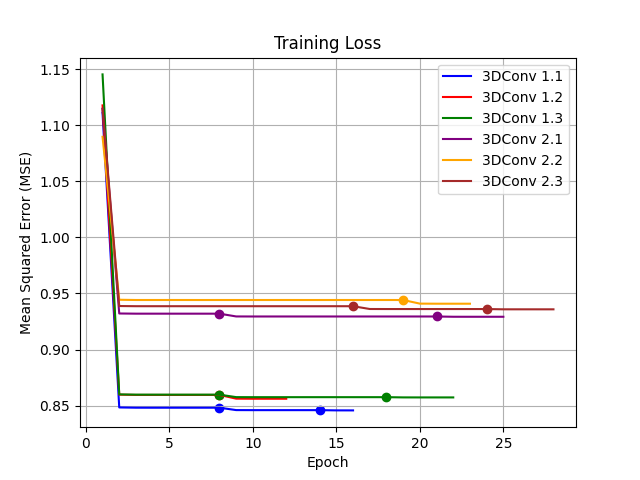
\includegraphics[width=0.32\textwidth]{./entities/pretrained/baseline/train_losses.png}
         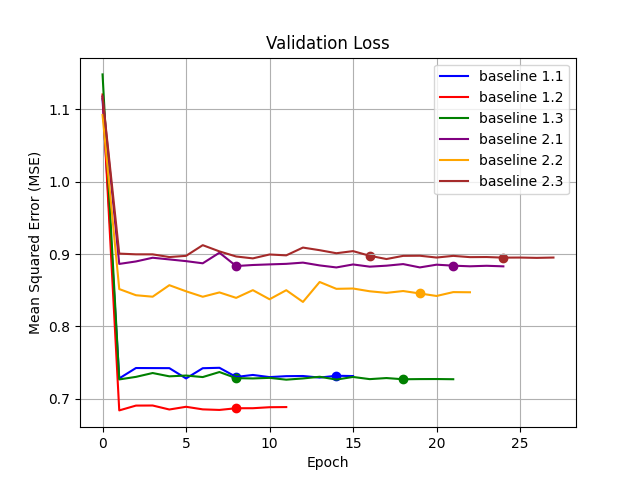
\includegraphics[width=0.32\textwidth]{./entities/pretrained/baseline/val_losses.png}
         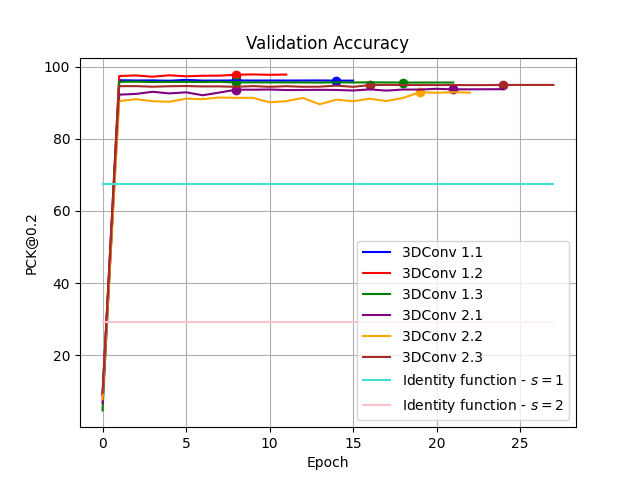
\includegraphics[width=0.32\textwidth]{./entities/pretrained/baseline/val_accs.png}
         \caption{Pretraining results of 3DConv.}
     \end{subfigure}
    \hfill

    \begin{subfigure}[b]{\textwidth}
        \centering
        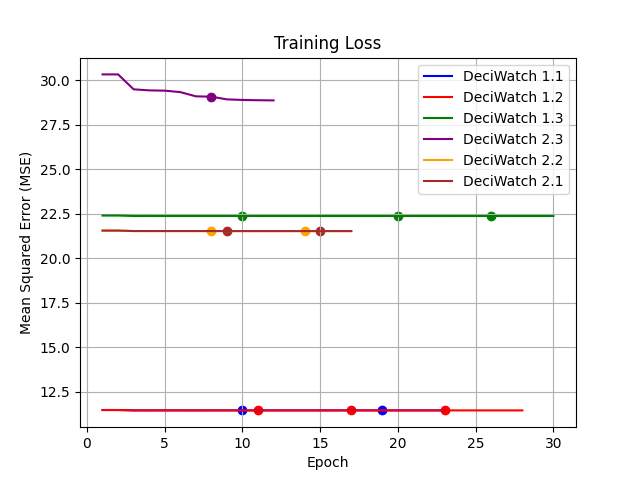
\includegraphics[width=0.32\textwidth]{./entities/pretrained/deciwatch/train_losses.png}
        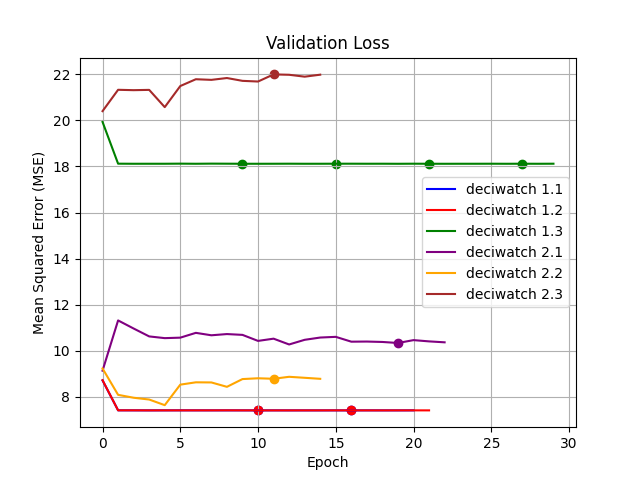
\includegraphics[width=0.32\textwidth]{./entities/pretrained/deciwatch/val_losses.png}
        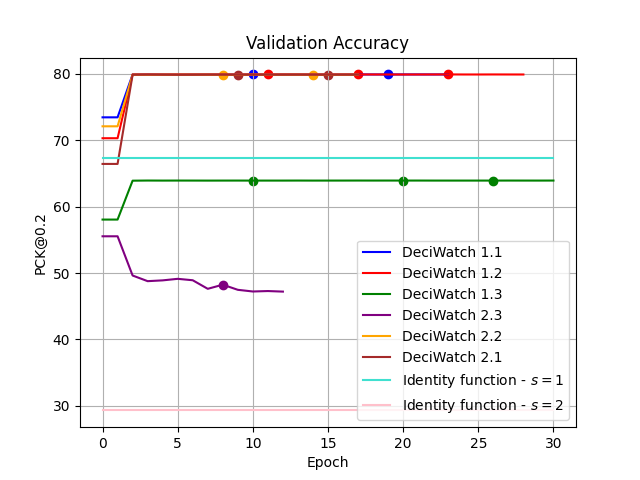
\includegraphics[width=0.32\textwidth]{./entities/pretrained/deciwatch/val_accs.png}
        \caption{Pretraining results of DeciWatch.}
    \end{subfigure}
   \hfill

   \begin{subfigure}[b]{\textwidth}
    \centering
    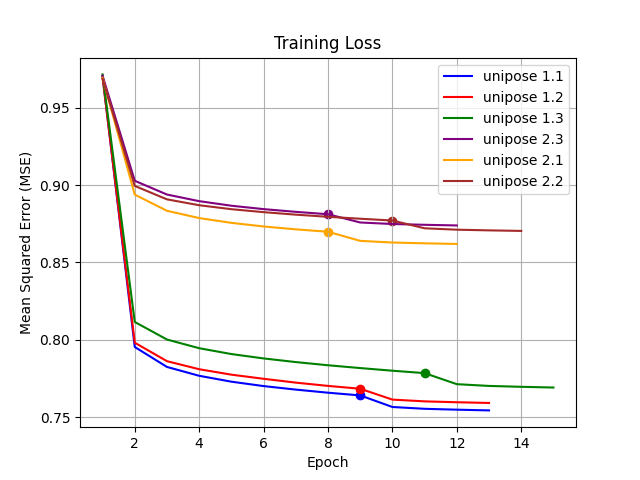
\includegraphics[width=0.32\textwidth]{./entities/pretrained/unipose/train_losses.png}
    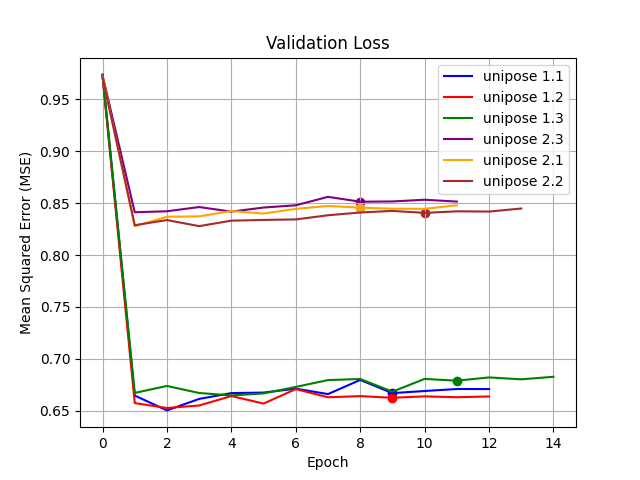
\includegraphics[width=0.32\textwidth]{./entities/pretrained/unipose/val_losses.png}
    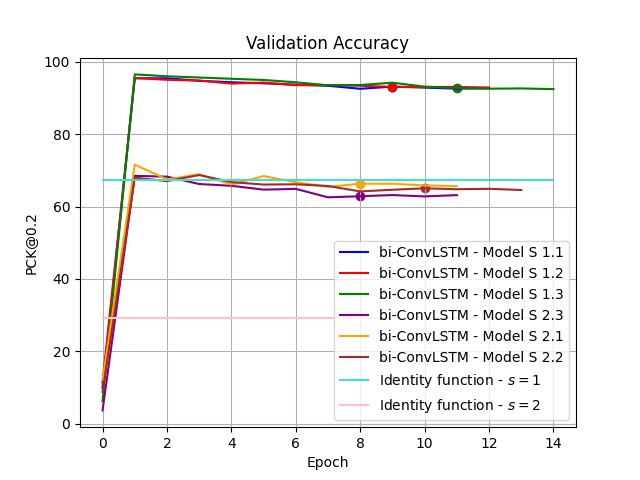
\includegraphics[width=0.32\textwidth]{./entities/pretrained/unipose/val_accs.png}
    \caption{Pretraining results of the bi-ConvLSTM Model S.}
    \end{subfigure}
    \hfill

    \begin{subfigure}[b]{\textwidth}
        \centering
        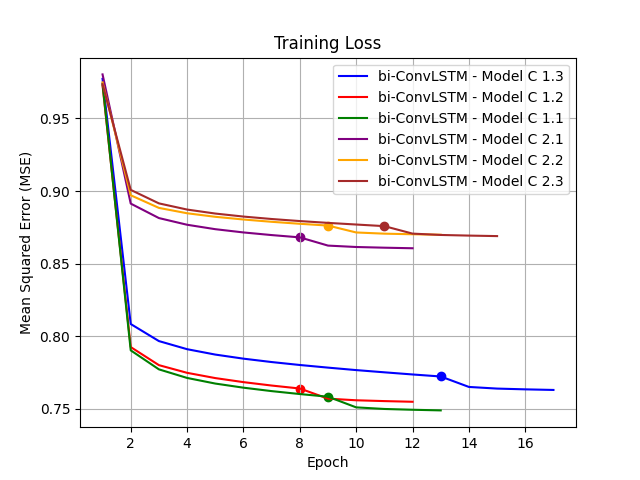
\includegraphics[width=0.32\textwidth]{./entities/pretrained/unipose2/train_losses.png}
        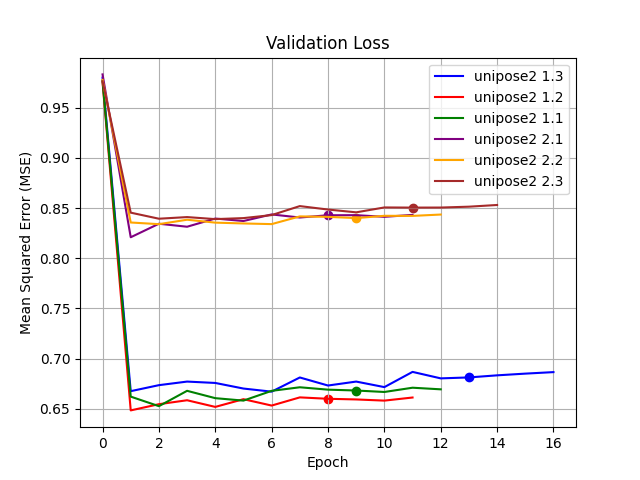
\includegraphics[width=0.32\textwidth]{./entities/pretrained/unipose2/val_losses.png}
        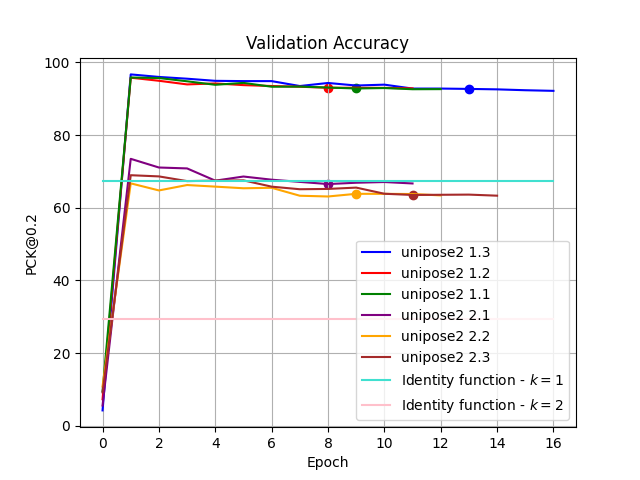
\includegraphics[width=0.32\textwidth]{./entities/pretrained/unipose2/val_accs.png}
        \caption{Pretraining results of the bi-ConvLSTM Model C.}
    \end{subfigure}
    \hfill
    
    \caption{Evolution of the training loss, validation loss and validation PCK@0.2 accuracy of the 24 models during training, as well as the validation PCK@0.2 accuracy of the identity function of the two datasets. The dots indicates a reduction of learning rate. First row: 3DConv. Second row: DeciWatch. Third row: bi-ConvLSTM Model S. Fourth row: bi-ConvLSTM Model C.}
    \label{fig:pretraining_res}
\end{figure}

We have in Figure \ref{fig:pretraining_res} visualized the evolution of the training loss, validation loss and validation PCK@0.2 accuracy for our 24 models. Each model is delt two numbers seperated by a dot such that it follows a $x.y$-format (for instance, '$2.3$'), indicating what type of shifing-scalar and experiment it refers to. $x$ indicates what shifting-scalar was used when shifting the input keypoints, and $y$ indicates which of the three experiments from section \ref{subsubsec:training_details} the run belongs to. Each plot has at least one dot, which indicates the reduction of the learning rate due to five consecutive epochs without beating the minimum validation loss.
\\
\\
By comparing the validation accuracies of the various models against the identity function we see, that all of the models, except for DeciWatch 1.3, do learn to somewhat denoise the input data. The simple 3DConv seems to be the architecure that generally delivers the greatest results, whereas DeciWatch is generally the architecure that delivers the worst results. Further, the two architectures that are based on bidirectional convolutional LSTMs have close to no difference in their performance, indicating that our raised concern about one of the architectures not being able to prioritize one LSTM-branch over the other is not as great as we hypothesized it to be.
\\
\\
From the figure we can see, that generally the reduction of the learning rate has an effect on the training loss, as generally the training loss is immediately decreased after a reduction of the learning rate. However, the same cannot be said about the validation loss and accuracy, as these do not immediately decrease after the learning rate has been reduced. Often, the training even terminates before a second reduction of the learning rate takes place, indicating the missing effect of the learning rate reduction on the validation loss.
\\
\\
Further, we can clearly see the effects of the shifting-scalar on the training of the models, as all of the models performs better on the dataset with a low shifting-scalar, than on their corresponding counterpart with a higher shifting-sclar. DeciWatch $1.3$ and DeciWatch $2.3$ do however seems to be struggling quite a bit, as the validation accuracies of these models are much lower than the other DeciWatch models with the same noise-scalar.

\subsection{Test Results}
\label{subsec:pretrain_test_res}
\begin{table}[htbp]
    \begin{tabular}{c||ccc|ccc|ccc}
        \hline
        Accuracy metric & \multicolumn{3}{c}{PCK@0.05} & \multicolumn{3}{c}{PCK@0.1} & \multicolumn{3}{c}{PCK@0.2} \\
        \hline
        Mean threshold distance (px)* & \multicolumn{3}{c}{1.11} & \multicolumn{3}{c}{2.23} & \multicolumn{3}{c}{4.46} \\
        \hline
        Experiment & 1.1 & 1.2 & 1.3 & 1.1 & 1.2 & 1.3 & 1.1 & 1.2 & 1.3 \\
        \hline
        \hline
        Identity function & 6.95 & 6.95 & 6.95 & 25.7 & 25.7 & 25.7 & 67.4 & 67.4 & 67.4 \\
        3DConv & 1.84 & 20.5 & 0.67 & 30.6 & 58.5 & 23.8 & \textbf{96.6} & \textbf{98.0} & 96.3 \\
        DeciWatch & \textbf{51.4} & \textbf{51.4} & \textbf{44.5} & 64.6 & 64.6 & 51.5 & 80.2 & 80.2 & 64.2 \\
        bi-ConvLSTM Model S & 27.8 & 31.1 & 33.8 & 68.4 & 71.0 & \textbf{72.5} & 95.7 & 95.8 & 96.7\\
        bi-ConvLSTM Model C & 29.5 & 31.7 & 31.8 & \textbf{69.5} & \textbf{71.3} & 71.8 & 96.1 & 96.1 & \textbf{96.9} \\
        \hline
    \end{tabular}
    \caption{Testing accuracies of the various developed models for shifting-scalar $s = 1$. All the accuracies are in percentage. *: The mean maximum distance between the predicted keypoint and corresponding groundtruth keypoint for the prediction to count as being correct, measured in the heatmap coordinate system.}
    \label{tab:pretrain_test_accs_1}
\end{table}

\begin{table}[htbp]
    \begin{tabular}{c||ccc|ccc|ccc}
        \hline
        Accuracy metric & \multicolumn{3}{c}{PCK@0.05} & \multicolumn{3}{c}{PCK@0.1} & \multicolumn{3}{c}{PCK@0.2} \\
        \hline
        Mean threshold distance (px)* & \multicolumn{3}{c}{1.11} & \multicolumn{3}{c}{2.23} & \multicolumn{3}{c}{4.46} \\
        \hline
        Experiment & 2.1 & 2.2 & 2.3 & 2.1 & 2.2 & 2.3 & 2.1 & 2.2 & 2.3 \\
        \hline
        \hline
        Identity function & 1.84 & 1.84 & 1.84 & 7.75 & 7.75 & 7.75 & 29.3 & 29.3 & 29.3 \\
        3DConv & 0.80 & 2.40 & 0.11 & 21.6 & 27.6 & 16.8 & \textbf{94.2} & \textbf{91.8} & \textbf{95.5} \\
        DeciWatch & \textbf{51.2} & \textbf{51.2} & \textbf{10.3} & \textbf{64.4} & \textbf{64.4} & 24.4 & 80.2 & 80.2 & 50.3 \\
        bi-ConvLSTM Model S & 10.5 & 11.6 & 10.1 & 31.1 & 33.4 & 29.5 & 68.5 & 67.8 & 69.6 \\
        bi-ConvLSTM Model C & 12.5 & 12.0 & 9.63 & 36.4 & 32.5 & \textbf{29.8} & 74.6 & 65.5 & 70.0 \\
        \hline
    \end{tabular}
    \caption{Testing accuracies of the various developed models for shifting-scalar $s = 2$. All the accuracies are in percentage. *: The mean maximum distance between the predicted keypoint and corresponding groundtruth keypoint for the prediction to count as being correct, measured in the heatmap coordinate system.}
    \label{tab:pretrain_test_accs_2}
\end{table}

\noindent We have in Table \ref{tab:pretrain_test_accs_1} and Table \ref{tab:pretrain_test_accs_2} illustrated the results of testing the epoch of each model that yielded the best validation PCK$@0.2$ accuracy.
\\
\\
For shifting-scalar $s = 1$ we see, that DeciWatch is the architecure that yields the best results for PCK$@0.05$, however, for PCK$@0.2$ DeciWatch actually tends to be the worst performing model. Further, as stated in section \ref{subsec:pretrain_train_val_res} DeciWatch 1.3 does perform worse than the identity function when considering PCK$@0.2$, however, for both PCK$@0.05$ and PCK$@0.1$ DeciWatch 1.3 completely outperforms the identity function, hence why it actually does learn to denoise the data, unlike what we stated in section \ref{subsec:pretrain_train_val_res} where we just looked at the validation PCK$@0.2$ accuracy. Generally, most of the predicitons of DeciWatch that are considered correct, are actually very close to the groundtruth, however the predictions that are incorrect are pretty far away from their corresponding groundtruth location.
\\
\\
On the other hand, the simple 3DConv seems to be the architecture that generally performs the worst for PCK$@0.05$ and PCK$@0.1$, and actually the architecture that performs the best for PCK$@0.2$, except for run 1.3, where the two bidirectional convolutional LSTM based models actually outperforms it. Thus, 3DConv is very good at inferencing a rough estimate of the position of the keypoints, however, the exact position of these predictions are generally incorrect.
\\
\\
Generally, the bidirectional convolutional LSTMs yield some decent results, as the predicitons of these models are always pretty far away from the worst-performing model for any of the three used accuracy metrics, and for PCK$@0.1$ they even seem to yield the best results of the four architectures. Similarly to the validation results, the test results do only indicate a minor performance differences between the two different types of bidirectional convolutional LSTMs in favor of the bi-ConvLSTM Model C. Likewise, similarly to the validation results, the test results indicate a major effect of a low frame rate for DeciWatch. 
\\
\\
If we compare the performances of the models on experiment 2 against their performances on experiment 1 we see, that all arhcitectures, except for DeciWatch, performs better on experiment 2 than they do on experiment 1. This is especially true for 3DConv, whose run on experiment 2 completely outperforms its run on experiment 1. On the other hand, if we compare the results of experiment 3 against the results of experiment 1 we see, that both 3DConv and DeciWatch perform worse on experiment 3 than they do on experiment 1. However, the two archtectures that are based on a bidirectional convolution LSTM actually continuously performs better in experiment 3 than they do in experiment 1, making us believe that the added context when decreasing the frame rate, actually help these models.
\\
\\
Generally, the testing results of shifting-scalar $s = 2$ follow the same pattern with some minor differences. If we consider the results of PCK$@0.2$, 3DConv is now the architecture that always yields the best results - and by a large margin, but it is on the other hand completely outperformed by the other models when considering PCK$@0.05$. This indicates, that the architecture can still yield decent rough estimations of the keypoints when a lot of noise is added, however, it does also indicate, that the exact position of these keypoints are very much effected by the level of noise. Further, its results in experiment 2 do not any longer outperform its results in experiment 1 when considering PCK$@0.2$, as it was the case for shifting-scalar $s = 1$.

\begin{table}[htbp]
    \begin{adjustbox}{center}
        \begin{tabular}{c||ccc|ccc|ccc|ccc|c}
            \hline
            & \multicolumn{3}{c}{3DConv} & \multicolumn{3}{c}{DeciWatch} & \multicolumn{3}{c}{\begin{tabular}[c]{@{}c@{}}bi-ConvLSTM\\Model S\end{tabular}} & \multicolumn{3}{c}{\begin{tabular}[c]{@{}c@{}}bi-ConvLSTM\\Model C\end{tabular}} & Total \\ 
            \hline
            Experiment & 1.1 & 1.2 & 1.3 & 1.1 & 1.2 & 1.3 & 1.1 & 1.2 & 1.3 & 1.1 & 1.2 & 1.3 & \\
            \hline
            \hline
            Nose & 30.4 & 44.3 & 26.5 & 68.9 & 68.0 & 54.1 & 80.6 & 67.7 & 81.4 & 74.9 & 73.3 & 70.1 & 61.7 \\
            Ear & 29.4 & 43.8 & 24.9 & 69.6 & 69.6 & 55.2 & 76.5 & 73.2 & 76.2 & 74.9 & 75.2 & 71.5 & 61.7 \\
            Shoulder & 34.0 & 71.3 & 29.4 & 68.1 & 68.1 & 53.5 & 65.2 & 72.0 & 71.4 & 70.9 & 77.0 & 69.4 & 62.5 \\
            Elbow & 31.1 & 68.3 & 24.0 & 62.7 & 62.7 & 49.4 & 71.9 & 79.0 & 68.0 & 67.6 & 71.9 & 83.6 & 61.7 \\
            Wrist & 26.5 & 45.3 & 19.8 & 59.8 & 59.8 & 48.3 & 70.5 & 70.4 & 66.8 & 68.6 & 70.7 & 74.6 & 56.8 \\
            Hip & 34.3 & 84.3 & 24.4 & 63.6 & 63.6 & 50.1 & 65.2 & 65.6 & 57.4 & 67.1 & 62.1 & 56.3 & 57.8 \\
            Knee & 33.7 & 65.2 & 25.1 & 59.5 & 59.5 & 48.0 & 73.9 & 69.2 & 66.8 & 61.9 & 69.0 & 73.2 & 58.8 \\
            Ankle & 25.4 & 37.2 & 17.6 & 58.9 & 58.9 & 48.3 & 80.1 & 69.4 & 66.1 & 73.1 & 72.2 & 75.2 & 56.9 \\
            \hline
            Total & 30.6 & 58.5 & 23.8 & 64.6 & 64.6 & 51.5 & 68.4 & 71.0 & 72.5 & 69.5 & 71.3 & 71.8 & \\
            \hline
        \end{tabular}
    \end{adjustbox}
    \caption{Keypoint-specific testing PCK@0.1-accuracies of the various models for shifting-scalar $s = 1$. All the accuracies are in percentage.}
    \label{tab:pretrain_kpts_test_accs_10_1}
\end{table}

\begin{table}[htbp]
    \begin{adjustbox}{center}
        \begin{tabular}{c||ccc|ccc|ccc|ccc|c}
            \hline
            & \multicolumn{3}{c}{3DConv} & \multicolumn{3}{c}{DeciWatch} & \multicolumn{3}{c}{\begin{tabular}[c]{@{}c@{}}bi-ConvLSTM\\Model S\end{tabular}} & \multicolumn{3}{c}{\begin{tabular}[c]{@{}c@{}}bi-ConvLSTM\\Model C\end{tabular}} & Total \\ 
            \hline
            Experiment & 1.1 & 1.2 & 1.3 & 1.1 & 1.2 & 1.3 & 1.1 & 1.2 & 1.3 & 1.1 & 1.2 & 1.3 & \\
            \hline
            \hline
            Nose & 20.5 & 20.5 & 17.3 & 67.9 & 22.2 & 41.8 & 75.8 & 36.2 & 29.1 & 32.8 & 35.2 & 25.5 & 35.4 \\
            Ear & 22.5 & 29.7 & 18.8 & 69.1 & 18.6 & 47.9 & 80.3 & 46.9 & 42.7 & 47.9 & 49.4 & 42.4 & 43.0 \\
            Shoulder & 22.4 & 30.5 & 17.0 & 68.1 & 13.3 & 32.2 & 74.7 & 26.3 & 23.3 & 32.8 & 31.5 & 21.0 & 32.8 \\
            Elbow & 22.5 & 32.0 & 16.5 & 62.7 & 14.1 & 19.3 & 58.2 & 33.9 & 21.1 & 27.2 & 31.1 & 27.1 & 30.5 \\
            Wrist & 21.5 & 26.9 & 17.1 & 59.7 & 34.2 & 35.5 & 69.4 & 37.1 & 32.3 & 39.8 & 33.1 & 33.5 & 36.7 \\
            Hip & 22.4 & 27.9 & 16.3 & 63.5 & 16.8 & 19.9 & 64.7 & 26.5 & 32.1 & 35.2 & 22.2 & 30.3 & 31.5 \\
            Knee & 19.9 & 25.5 & 15.4 & 59.5 & 24.2 & 23.4 & 60.1 & 28.2 & 16.1 & 26.0 & 21.0 & 13.2 & 27.7 \\
            Ankle & 21.0 & 24.5 & 16.2 & 58.8 & 47.5 & 35.6 & 69.4 & 34.1 & 40.0 & 48.6 & 39.4 & 43.7 & 39.9 \\
            \hline
            Total & 21.6 & 27.6 & 16.8 & 64.4 & 64.4 & 24.4 & 31.1 & 33.4 & 29.5 & 36.4 & 32.5 & 29.8 & \\
            \hline
        \end{tabular}
    \end{adjustbox}
    \caption{Keypoint-specific testing PCK@0.1-accuracies of the various models for shifting-scalar $s = 2$. All the accuracies are in percentage.}
    \label{tab:pretrain_kpts_test_accs_10_2}
\end{table}

\noindent We have further in Table \ref{tab:pretrain_kpts_test_accs_10_1} and Table \ref{tab:pretrain_kpts_test_accs_10_2} written the keypoint-specific testing PCK$@0.1$ accuracies of these models. For the keypoint-specific testing PCK$0.05$ and PCK$0.1$ accuracies of the models, see Table \ref{tab:pretrain_kpts_test_accs_05_1}-\ref{tab:pretrain_kpts_test_accs_20_2} in the appendix.
\\
\\
Looking at Table \ref{tab:pretrain_kpts_test_accs_10_1} we see, that the models with shifting-scalar $s = 1$ generally perform the best on the ears and shoulders, whereas they perform the worst the wrists and ankles. The models in Table \ref{tab:pretrain_kpts_test_accs_10_2} tells another story, as instead of performing the worst on the ankles and wrists, the elbows and knees are now the most difficult keypoints, and the ears, nose and ankles are now the least difficult keypoints.

\subsection{Technical Details}
\label{sec:pretrain_tech_details}
All models were trained and evaluated on a shared GPU cluster using a 24GB NVIDIA Titan RTX and an Intel(R) Xeon(R) Gold 6248 CPU @ 2.50GHz. All models were implemented in Python version 3.9.9 using PyTorch 2.0.0. 3DConv took about 60 minutes per epoch, DeciWatch about 86 minutes per epoch, the bi-ConvLSTM Model S about 75 minutes per epoch, and the bi-ConvLSTM Model C about 88 minutes per epoch.

\end{document}